% Based on the user-supplied bare_jrnl_new_sample4.tex.
% IEEEtran's normal journal typography and page geometry are retained.
\documentclass[letterpaper,journal]{IEEEtran}
\usepackage[T1]{fontenc}
\usepackage{amsmath,amssymb,amsfonts}
\usepackage{array,booktabs,multirow}
\usepackage{graphicx}
\usepackage{cite}
\usepackage{url}
\usepackage{stfloats}
\usepackage[hidelinks]{hyperref}
\graphicspath{{figures/}}
\hyphenation{net-work net-works coun-ter-fac-tual}
\newcommand{\method}{CFCMT}
\newcommand{\R}{\mathbb{R}}
\newcommand{\ind}{\mathbf{1}}
\DeclareMathOperator*{\argmin}{arg\,min}
\DeclareMathOperator*{\argmax}{arg\,max}
\DeclareMathOperator{\range}{range}
\DeclareMathOperator{\median}{median}
\newcommand{\sourcecommit}{61e8a81e10c058cf07125efe86f2a8c8e2dd1c18}
\hypersetup{pdftitle={CFCMT: Structured Action-Cost Transfer for Traffic Signal Control},pdfsubject={IEEE T-ITS manuscript; author information pending},pdfauthor={}}
\begin{document}
\title{CFCMT: Structured Action-Cost Transfer\\for Traffic Signal Control}
% T-ITS uses single-anonymous review. Supply the real author list here;
% do not use 'authors withheld for review' for a submission to this journal.
\author{Author information to be completed before submission}
\markboth{Manuscript prepared for IEEE Transactions on Intelligent Transportation Systems}%
{CFCMT: Structured Action-Cost Transfer for Traffic Signal Control}
\maketitle
\begin{abstract}
Road networks differ in junction layout, traffic demand, and available signal phases. A transferred controller must compare phase choices under these different conditions. We study a supervised transfer method that learns the cost difference between actions applied to the same simulated traffic state. A predictor restricted to local traffic features provides a reference, while a second predictor compares every pair of feasible phases. Development uses 18 networks in seven groups, followed by evaluation on two external networks. The final controller selects source-group components or a target anchor using target action labels and eight closed-loop development seeds, then freezes its predictors and execution guard. The complete comparison comprises 1,344 one-hour simulations across six controllers, four scenarios, and 56 paired seeds. Mean city-wise relative waiting decreases by 2.42\% against MaxPressure (95\% interval for the reduction, 0.66--4.58\%), with 40 of 56 seed means favorable. Against PhasePressure, the reduction is 1.91\%, although its interval crosses zero. Relative waiting also decreases by 2.30\% against the target anchor and 9.40\% against the dense linear residual model. The selected controller uses an Atlanta component in Jinan and the target anchor in Los Angeles. These results support structured action prediction and the tested source-selection procedure on the two target networks, with all adaptation and selection completed before evaluation.
\end{abstract}

\begin{IEEEkeywords}
Modelling and simulation, optimization and control, road transportation, traffic networks, traffic signal control, transfer learning.
\end{IEEEkeywords}
\section{Introduction}
\IEEEPARstart{A}{traffic} signal controller that works at one junction may make poor decisions at another. The number and ordering of phases can change, downstream roads may have different capacities, and the same queue length can call for a different action under a different demand pattern. These changes make cross-network deployment a more demanding test than evaluating a controller on new random seeds of the network used for training. For an operator, the practical question is whether experience from other networks improves decisions at the new location after a limited amount of local preparation.

Many signal-control methods learn a policy or value function from interaction with a simulator. Others predict future traffic and choose an action from those predictions. In either case, the decision depends on how the available actions compare. Predicting the absolute traffic state accurately is useful only to the extent that the prediction distinguishes the consequences of competing phases. An error shared by every candidate can be large without changing the preferred action; a small error in the difference between two candidates can reverse the decision.

This observation motivates a narrower prediction task. We restore the same simulated traffic state, try each feasible phase, and measure the difference in the resulting short-horizon costs. The learner then predicts these within-state differences. This construction removes cost components common to all candidates and avoids assigning a fixed output coordinate to each phase identity. It does not remove errors that affect actions differently, and it does not establish that a short-horizon ranking will remain useful after the controller changes the traffic state through repeated decisions.

We investigate this approach through Causal-Factored Cross-City Model Transfer (\method). Each source-group component combines two supervised predictors: a restricted predictor that compares each candidate with a pressure-based reference, and a pairwise predictor that compares every feasible pair. The second predictor is constrained so that reversing the order of a comparison reverses its sign. Component blend settings are fixed before source selection. Target development rollouts select the source weights and execution guard. The fitted controller subsequently scores feasible phases from the observed traffic state, without online model updates or counterfactual simulation at each decision.

The study addresses three questions. First, does the selected controller reduce waiting relative to the target anchor and dense linear residual baseline? Second, does selecting source components improve on equal source weights? Third, how does the frozen controller compare with pressure rules on the same target scenarios? Together, these comparisons assess source selection and the closed-loop performance of the resulting controller.

We develop the method on 18 networks in seven groups and evaluate it on external Los Angeles and Jinan benchmark networks. The final controller selects source-group components or a target anchor using target development runs, then freezes both its predictor and execution guard. The main comparison tests this frozen source selector on 56 paired seeds.

The contributions are threefold. We formulate transfer around matched phase-cost differences and give the associated invariance and ranking properties. We implement a restricted predictor, an antisymmetric pairwise predictor, and a source-selection procedure that chooses a fitted component or target anchor before deployment. We evaluate the frozen controller against learned and pressure baselines on matched target simulations, reporting both overall and city-specific performance.

\section{Related Work}
\subsection{Traffic structure in signal control}
Max-pressure control chooses service using upstream and downstream queue imbalance. Its stability results hold under the assumptions of the underlying traffic model \cite{varaiya2013maxpressure}; they do not automatically extend to every microscopic implementation. PressLight and MPLight use pressure-related representations or objectives in learned controllers \cite{wei2019presslight,chen2020thousandlights}. The flipping- and rotation-invariant all-phase (FRAP) model represents pairwise competition between phases and exploits symmetry among traffic movements \cite{zheng2019frap}, while CoLight represents cooperation between intersections \cite{wei2019colight}. These studies motivate using traffic structure in the state and action representations. Our comparison also retains deterministic pressure policies, because improvement over another learned model alone does not establish an operational advantage.

\subsection{Transfer across networks and simulators}
MetaLight learns an initialization that can be adapted with target experience \cite{zang2020metalight}. General Scenario-Agnostic (GESA) reinforcement learning provides a common representation for heterogeneous signal-control scenarios \cite{jiang2024gesa}, while X-Light learns cross-city representations from decision trajectories \cite{jiang2024xlight}. CrossLight explicitly combines offline source training with online target fine-tuning \cite{sun2024crosslight}. Their target interaction and adaptation requirements differ from ours: we use labelled target simulator interventions and separate target development rollouts before deployment, then keep the deployed model fixed. Their published results cannot be substituted for a comparison under this information setting.

Simulator mismatch creates a related but distinct problem. Dynamics-Aware Hybrid Offline-and-Online Reinforcement Learning (H2O) and its extension, An Improved Framework for Hybrid Offline-and-Online Reinforcement Learning with Dynamics Gaps (H2O$^+$), combine fixed data with simulator interaction while addressing discrepancies in the dynamics \cite{niu2022h2o,niu2023h2oplus}. Grounded action transformation instead modifies actions to reduce the simulator-to-target discrepancy \cite{da2023ugat}. Our residual baseline is a supervised robust linear estimator. Our training and evaluation also use the same simulation engine, so the study concerns cross-network adaptation in simulation rather than transfer to a physical signal system.

\subsection{Mechanisms and decision-relevant prediction}
Work on causal representation learning motivates decomposing systems into mechanisms that can change separately across environments \cite{bengio2019meta,scholkopf2021causal}. Factored adaptation applies related ideas to non-stationary reinforcement learning \cite{feng2022factored}. Here, this motivation leads to predefined traffic features and controlled interventions within a simulator. We do not infer a causal graph from field observations. Our prediction target is the relative consequence of phase choices, and the final estimator uses gradient-boosted trees \cite{friedman2001greedy,pedregosa2011scikit}. This distinction matters: the evidence concerns the implemented predictors and control protocol, not the validity of a discovered causal structure.

\section{Problem and Target Information}
Consider a traffic network $n$ with several signalized intersections. At a decision time, let $s$ denote the observed traffic and signal state and let $\mathcal A(s)$ be the feasible green stages at the focal intersection. The controller chooses a stage every 10~s. A shared signal executor implements the requested stage while enforcing the signal program's minimum-green, yellow, and all-red requirements. This separates phase selection from the physical transition sequence.

For training, the complete Simulation of Urban MObility (SUMO) state is available \cite{lopez2018microscopic}. Let $g$ index a saved state $s_g$, with feasible actions $\mathcal A_g=\mathcal A(s_g)$, and let $Y_g(a)$ be the measured cost of applying action $a$ at that state under a specified continuation policy. An \emph{action group} contains the outcomes for all $a\in\mathcal A_g$. At deployment, these outcomes are unavailable: only state-derived features and the previously fitted model can be used to rank the actions. The objective is low waiting time over the full control run, assessed separately from the short-horizon training cost.

The available information consists of a source-network action bank, the target network and demand files, target action groups and development outcomes collected in simulation, and current target traffic observations during operation. The target simulator is not fitted to field trajectories. Nevertheless, its action outcomes are labelled target data. We call this \emph{predeployment target adaptation}: all fitting and model selection finish before the evaluation rollouts. It neither requires online learning during those rollouts nor provides evidence of zero-shot or real-world transfer.
Fig.~\ref{fig:workflow} summarizes these information roles.

\begin{figure*}[!t]
\centering
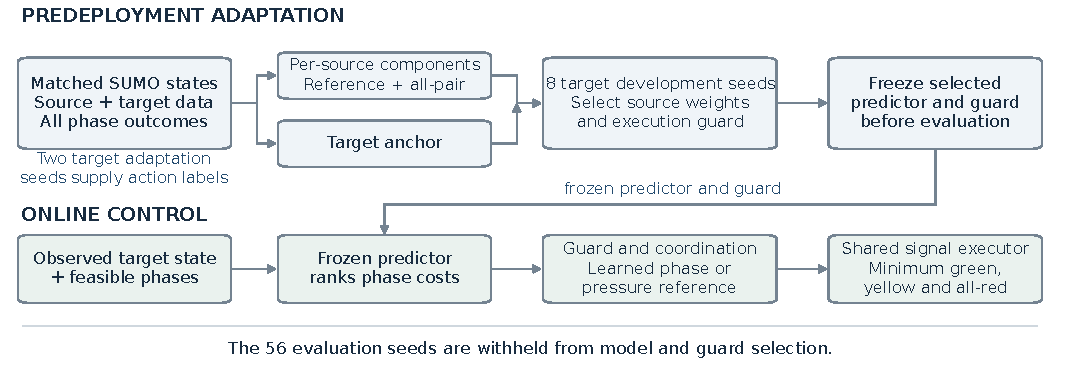
\includegraphics[width=\textwidth]{method_workflow.pdf}
\caption{Learning and deployment use different information. Matched simulator interventions provide source and target training outcomes. Two adaptation seeds supply target action labels; eight separate target development seeds select source weights and the execution guard. Deployment uses frozen predictors, the selected guard, sparse coordination, and current observations; evaluation outcomes are not used to select the controller.}
\label{fig:workflow}
\end{figure*}

\section{Learning to Compare Phase Choices}
The following score construction defines each source-group component. The final controller can also select a target anchor, as described in Section~\ref{sec:source-selector}.
\subsection{Collecting matched action outcomes}
After a 60-s warm-up, we save the simulator state and the states of all signal executors. Each candidate phase starts from an exact restoration of this snapshot. The focal signal requests that phase for one 10-s interval and then follows PhasePressure for five more intervals. Other signals follow PhasePressure throughout. Thus, each label measures one intervention followed by a common continuation, rather than a complete rollout of the learned controller.

The branch cost is the mean active-plus-pending vehicle load per controlled lane:
\begin{equation}
 Y_g(a)=\frac{1}{60}\sum_{\tau=1}^{60}
 \frac{N_{\mathrm{active}}(\tau)+N_{\mathrm{pending}}(\tau)}{L_n},
 \label{eq:cost}
\end{equation}
In \eqref{eq:cost}, samples are one second apart and $L_n$ counts distinct incoming lanes controlled by all signals in the network. $N_{\mathrm{active}}(\tau)$ and $N_{\mathrm{pending}}(\tau)$ count active and insertion-pending vehicles across that network at branch second $\tau$, starting from $s_g$ with action $a$. Pending vehicles are included so that restricting insertion does not appear to reduce the training cost. Collection checks deterministic replay and rejects teleports. If any candidate has a junction collision, the whole action group is excluded; the retained groups therefore contain all candidate outcomes. This screening concerns the training groups and does not remove adverse runs from closed-loop evaluation.

A generalized pressure rule supplies a reference phase $r_g$. Its parameters are selected on source networks. The reference used for the external targets maximizes $q_{\mathrm{green}}(a)-0.02o_{\mathrm{down}}(a)$, where the two features summarize the served-queue proxy and downstream occupancy. For lane $\ell$, the queue proxy is $q_\ell=N_{\mathrm{halted},\ell}+0.35N_{\mathrm{vehicles},\ell}+0.025o_\ell$, where $N_{\mathrm{halted},\ell}$ and $N_{\mathrm{vehicles},\ell}$ count halted and total lane vehicles and $o_\ell$ is the simulator-reported lane occupancy; $q_{\mathrm{green}}$ sums the proxy over served incoming lanes. This reference defines the origin of the learned scores. It differs from the PhasePressure continuation, which maximizes the served-queue proxy alone.

Let $c_g(a)=Y_g(a)-Y_g(r_g)$. The normalized label and offline regret are
\begin{align}
 \sigma_g&=\max\{\max_aY_g(a)-\min_aY_g(a),10^{-8}\},\nonumber\\
 z_g(a)&=c_g(a)/\sigma_g,\label{eq:label}\\
 R_g(\widehat a)&=\{Y_g(\widehat a)-\min_aY_g(a)\}/\sigma_g.
 \label{eq:regret}
\end{align}
The implemented scale also includes $10^{-6}$ times the 75th percentile of $|c_g(a)|$. Since the group includes $c_g(r_g)=0$, this extra term cannot exceed a nonzero group range; \eqref{eq:label} is the equivalent scale. No test outcome is needed at deployment: $\sigma_g$ normalizes training labels and evaluation regret, not the model's runtime input.

\subsection{Why compare costs within a state?}
Suppose that $Y_g(a)=b_g+\mu_g(a)+e_g(a)$, where $b_g$ is common to the candidates, $\mu_g(a)$ is the action-dependent cost component, and $e_g(a)$ is an action-dependent error. Subtracting the reference gives
\begin{equation}
 c_g(a)=\mu_g(a)-\mu_g(r_g)+e_g(a)-e_g(r_g).
 \label{eq:cancellation}
\end{equation}
The common term cancels. Adding a constant to every outcome also leaves $\sigma_g$, the labels, and the optimal action unchanged. Positive rescaling preserves the action ordering; it preserves the normalized values provided neither the original nor the rescaled range activates the numerical floor. These elementary properties motivate the target representation. They do not imply that $e_g(a)$ is small or that phase effects are invariant between networks.

\subsection{Restricted reference predictor}
The first predictor, $A_g(a)=A_\theta(s_g,a)$, with fitted parameters $\theta$, regresses $z_g(a)$ for non-reference actions and sets $A_g(r_g)=0$. It uses 29 predefined features describing aggregate traffic state, queues served or stopped by the candidate and reference, downstream load, pressure, switching, clearance, and overlap with the current phase. Network identity and unrestricted static context are excluded from its prediction inputs. These restrictions encode an engineering hypothesis about useful traffic variables; they are not a learned causal graph.

We fit histogram-based gradient-boosted trees with squared-error loss. A training domain denotes one geographical or synthetic network group; target examples form an additional domain during adaptation. Base sample weights give each domain equal weight and each action group equal weight within its domain. We then multiply by $\operatorname{clip}(|z_g(a)|,0.25,4)$ and apply capped sign balancing so that the fit does not simply favor the more frequent sign of action improvement. Here $\operatorname{clip}$ limits its first argument to the stated interval. The resulting weights are normalized to mean one. Because of these adjustments, the final total weights need not remain exactly equal across domains.

\subsection{Comparing every pair of phases}
The second predictor uses a common state vector $x_g\in\R^{23}$ and a phase feature vector $\phi_g(a)\in\R^{40}$. The state features include local traffic, time, elapsed green, queue concentration, and summaries of neighboring signals. Phase features describe demand served, downstream conditions, phase duration, transitions, and the affected road connections. For every unordered pair of actions $a_i,a_j$, training uses
\begin{equation}
 \bigl([x_g,\phi_g(a_i)-\phi_g(a_j)],\;
 t_{gij}=z_g(a_i)-z_g(a_j)\bigr).
 \label{eq:pairdata}
\end{equation}
Square brackets in \eqref{eq:pairdata} denote vector concatenation. The reverse pair is added with the opposite target. Pair weights give equal total weight to domains, to groups within a domain, and to unordered pairs within a group. The same regression family as the reference predictor is used.

At prediction, we enforce antisymmetry explicitly:
\begin{equation}
 \widehat\delta_{gij}=\frac{f_\psi(x_g,\phi_i-\phi_j)
 -f_\psi(x_g,\phi_j-\phi_i)}{2}.
 \label{eq:antisym}
\end{equation}
Here $f_\psi$ is the pairwise regressor with fitted parameters $\psi$, and $\phi_i$ abbreviates $\phi_g(a_i)$. With $K_g=|\mathcal A_g|\geq2$, the action scores are
\begin{align}
 \widetilde P_g(a_i)&=\frac{1}{K_g-1}\sum_{j\ne i}\widehat\delta_{gij},\nonumber\\
 P_g(a_i)&=\widetilde P_g(a_i)-\widetilde P_g(r_g).
 \label{eq:pairscore}
\end{align}
An intersection with only one available action requires no comparison. If all pair predictions are exact, substitution in \eqref{eq:pairscore} gives
\begin{equation}
 P_g(a_i)=\frac{K_g}{K_g-1}\{z_g(a_i)-z_g(r_g)\}.
 \label{eq:recovery}
\end{equation}
The factor is positive, so the action ranking is recovered. Its value is retained when combining the pairwise score with the reference predictor; the two score scales are not assumed identical.
Appendix~\ref{app:score-proofs} gives the derivations of \eqref{eq:cancellation} and \eqref{eq:recovery}.

Both predictors use learning rate 0.05, 100 boosting iterations, at most 15 leaves per tree, and $L_2$ regularization 10, with early stopping disabled. Minimum leaf sizes are 12 for the reference model and 20 for the pairwise model. These settings are fixed before external evaluation.

\subsection{Combining the predictors}
Each anchored source component uses a convex combination,
\begin{equation}
 S_g(a)=(1-\alpha_g)A_g(a)+\alpha_gP_g(a),\qquad
 \widehat a_g=\argmin_{a\in\mathcal A_g}S_g(a).
 \label{eq:blend}
\end{equation}
Component blend rules are fixed before source selection. The deployed Jinan component uses constant $\alpha_g=0.9$. The Los Angeles source candidates and equal-source comparator use the local rule in \eqref{eq:la-component-blend}, given in Appendix~\ref{app:score-proofs}; the final Los Angeles controller instead uses the target anchor described below.

The component predictors also return heuristic error scores. Let $e_A$ and $e_P$ be the 90th percentiles of absolute \emph{in-sample} residuals for the two models, floored at $10^{-6}$, and let $d_g$ be the distance to the closest training-network context after standardization by the domain-centroid spread. For non-reference actions, define
\begin{align}
 u_{A,g}(a)&=e_A(1+0.25d_g),\nonumber\\
 v_g(a_i)&=\frac{1}{K_g-1}\sum_{j\ne i}
 \left|\widehat\delta_{gij}-(\widetilde P_g(a_i)-\widetilde P_g(a_j))\right|,\nonumber\\
 u_{P,g}(a_i)&=(e_P+v_g(a_i))(1+0.25d_g).
 \label{eq:error_scores}
\end{align}
Both error scores in \eqref{eq:error_scores} are set to zero at the reference action. Context is used in these diagnostics, not in direct score prediction. The quantity $v_g$ measures disagreement between pair predictions and aggregated scores; because of the scaling in \eqref{eq:recovery}, it is not a pure measure of inconsistent preference cycles. Neither error score is an independently calibrated probability or confidence interval.

For the normalized regret in \eqref{eq:regret}, the component choice in \eqref{eq:blend} satisfies the general inequality $z_g(\widehat a_g)-\min_a z_g(a)\leq2\|S_g-z_g\|_\infty$. It follows by adding and subtracting the predicted scores at the selected and optimal actions (Appendix~\ref{app:score-proofs}). This bounds component action regret in terms of prediction error, before source selection and execution guarding.

\subsection{Source-group selection and deployment}
\label{sec:source-selector}
The final source selector fits a separate instance of the anchored predictor for each source group, using that group's examples together with the target adaptation groups with fixed blend settings. At zero source weight it uses the target anchor. That model uses 117 features and retains its original domain-scaled labels: contrasts are divided by the median positive action-group range in the same training domain, with a numerical floor, then clipped to $[-5,5]$. Its target regressor uses learning rate 0.05, 80 boosting iterations, at most seven leaves, minimum leaf size four, and $L_2$ regularization 16. Its target prediction weight is numerically almost one; a retained source prior can still resolve ties.

Selection uses eight target development seeds in three stages. First, each of seven source groups is tested at source weight 0.75 against the target anchor. The selected source is then tested at weights $\{0,0.25,0.5,0.75,1\}$. A source candidate is eligible only with at least 0.5\% mean waiting improvement, at most 1\% worst-seed regression, and no added collision or teleport incidents per seed. Eligible candidates minimize mean relative waiting change plus half its standard deviation and the positive part of the worst relative change; otherwise selection returns the target anchor. Finally, guard profiles with risk multipliers 0, 0.25, and 0.5 are compared with the selected unguarded controller. Eligible guards do not increase aggregate incidents or exceed 1\% worst-seed regression, and must reduce incidents or improve mean waiting by at least 0.5\%. Selection prioritizes fewer incidents, then the same waiting score; the unguarded controller remains available. All these choices precede the final evaluation.

The resulting Jinan controller uses the Atlanta component at source weight one and guard multiplier 0.5. Its error score is $(1-\alpha_g)u_{A,g}(a)+\alpha_g u_{P,g}(a)$. A learned phase replaces the generalized-pressure reference only when its predicted contrast plus 0.5 times this error score is negative and its normalized pressure deficit is at most one. The deficit is $\max\{\Pi(r_g)-\Pi(a),0\}/\max\{|\Pi(r_g)|,1\}$, where $\Pi$ is the generalized-pressure score defined above. Los Angeles selects zero source weight and the target anchor without this guard.

Learned departures from the pressure reference use sparse coordination. At each decision, a greedy selection admits mutually nonconflicting proposals on the signal conflict and routing graph. A five-interval cooldown gives a minimum 60-s gap between interventions at the same or conflicting signals, with 10-s decisions. Proposals that are blocked or not selected use the pressure reference. Pure MaxPressure and PhasePressure use the common phase executor without this learned-intervention coordinator. The predictors, source weights, guard, and coordination settings remain fixed throughout evaluation.

\section{Evaluation Design}
\subsection{Networks and simulator}
Experiments use SUMO 1.22.0 through \texttt{libsumo} \cite{lopez2018microscopic}. The source collection contains 18 networks, 317 controlled signals, and 6,076 non-internal lanes, grouped as in Table~\ref{tab:networks}. There are six geographical groups and one synthetic group. The collection draws on public signal-control benchmarks, including Reinforced Signal Control (RESCO) and LibSignal \cite{ault2021reinforcement,mei2022libsignal}.

The external targets are a four-signal Los Angeles corridor from LibSignal and a 12-signal Jinan network from the CoLight benchmark \cite{wei2019colight}. Jinan has three demand files on the same geometry. These inputs were distributed in CityFlow format \cite{zhang2019cityflow} and converted to SUMO, preserving demand, route continuity, phase identities, and protected versus permissive movements. A pre-evaluation execution check was used to detect conversion defects. These are benchmark representations of parts of cities, not calibrated city-wide digital twins.

\begin{table}[!t]
\caption{Network Inventory}
\label{tab:networks}
\centering
\begin{tabular}{lrrr}
\toprule
Group & Networks & Signals & Lanes\\
\midrule
Atlanta & 1 & 5 & 55\\
Cologne & 3 & 12 & 252\\
Hangzhou & 6 & 36 & 532\\
Ingolstadt & 3 & 32 & 2,227\\
New York & 1 & 196 & 2,562\\
Synthetic & 2 & 32 & 360\\
Salt Lake City & 2 & 4 & 88\\
\midrule
Source total & 18 & 317 & 6,076\\
\midrule
Los Angeles (target) & 1 & 4 & 157\\
Jinan (target) & 1 & 12 & 186\\
\bottomrule
\end{tabular}
\end{table}

\subsection{Separating development, adaptation, and tests}
The source bank used to fit the external models includes simulation seeds 2027, 3037, and 4047.

Target adaptation seeds 5057 and 6067 yield 165 complete action groups in Los Angeles and 911 in Jinan. Each group contains multiple alternative-action outcomes and should not be interpreted as one passive observation. Final evaluation outcomes are not used to tune the predictors, source weights, or guard.

Each closed-loop run lasts 3,600~s in total, including a 60-s warm-up. The final comparison uses four target scenarios and 56 paired seeds. The two cities receive equal weight; Jinan's three demands are first averaged within that city.

For the final source selector in Section~\ref{sec:source-selector}, static network context is repaired by tracing controlled movements through intermediate links to the nearest downstream signals, and context-dependent analytic priors are recomputed. The recorded action features and outcome labels remain unchanged. Models use all 165 Los Angeles or 911 Jinan adaptation groups. Eight separate target development seeds select the source group, source weight, and guard. Selection returns the target anchor without a guard for Los Angeles and the Atlanta component at weight one for Jinan, with constant blend weight 0.9 and guard multiplier 0.5. The target-anchor and equal-source comparators receive the same city-specific guard and sparse coordination as the selected controller. The latter averages predictions of the seven source-group components with equal weights. All choices are frozen before 56 paired evaluation seeds. Five controllers contribute 1,120 one-hour runs. MaxPressure is subsequently added as a fixed baseline on the same 56 seeds and four scenarios, giving 224 further runs and 1,344 in total. It uses the existing MaxPressure implementation, with no model refitting or parameter selection. All six methods share network files, phase executor, and decision timing. This protocol uses target closed-loop development outcomes in addition to the two adaptation seeds.

\subsection{Comparators and common execution}
The final comparison includes the frozen \method\ selector, the target anchor, an equal-weight mixture of the seven source components, a frozen dense linear residual model, PhasePressure, and MaxPressure. The implemented MaxPressure subtracts the downstream-queue proxy from the served-queue proxy. PhasePressure uses the served-queue proxy alone.

The dense linear model fits a correction to the analytic prior using the full local-feature and context vector. It uses domain-balanced robust ridge regression, with $L_2$ penalty 3, Huber parameter 1.5, and three robust-fitting iterations. It is fitted on the complete source bank and target adaptation data and remains frozen for the final comparison. The source-selection components instead use individual source groups and the same target adaptation data. The methods also differ in function class, normalization, and weighting. The comparison therefore tests complete estimator configurations; it does not isolate the effect of feature restrictions at matched model capacity.

All controllers share network and demand files. Learned and pressure controllers use the same candidate phase identities and phase executor. The executor reads the signal program's positive minimum-green duration; otherwise it uses up to 5~s, bounded by the phase duration and at least 1~s. Yellow and all-red durations use the corresponding program medians, with defaults of 3~s and 1~s. All-red is extended in one-second increments while the junction interior is occupied. These constraints are implementation safeguards, not a proof of collision-free control.

\subsection{Outcomes and uncertainty}
The primary outcome is average waiting time over all vehicles that depart during a run, including waiting accrued by unfinished trips up to the fixed endpoint. Waiting records and cumulative departure and arrival counts include the warm-up period. The measure avoids reporting only completed trips, but remains finite-horizon and excludes vehicles that never depart. System vehicle-hours sum one-second active-plus-pending vehicle counts from the warm-up endpoint through the simulation endpoint and divide by 3,600; the 60--3,600~s endpoints give 3,541 samples. Demand completion is $C_{\mathrm{arr}}/(C_{\mathrm{dep}}+N_{\mathrm{pending}}(T))$, where $C_{\mathrm{arr}}$ and $C_{\mathrm{dep}}$ are cumulative arrivals and departures at the simulation endpoint $T=3{,}600$~s. Simulator incidents are retained in the per-run exports. Together, these measures expose changes in insertion, network loading, and unfinished traffic.

For the 56-seed source-selection comparison, waiting is first averaged across scenarios within each city and seed. Relative change is then calculated against the comparator within each city, followed by equal averaging across cities and seeds. This registered mean of city-wise ratios differs from the ratio of pooled waiting means. The 95\% intervals use 20,000 paired seed-block bootstrap replicates. The four-comparator audit preceding the MaxPressure supplement uses Holm correction over 12 two-sided Wilcoxon tests. With MaxPressure added, the expanded report applies Holm correction over all 15 city or equal-city comparisons against five comparators. Those intervals are retained; the three supplemental MaxPressure intervals use NumPy's permuted congruential generator (PCG64) with seeds 20261030, 20261031, and 20261032 for Los Angeles, Jinan, and the equal-city effect, respectively, fixed before the new runs. All 56 seeds are retained.


\section{Results}
\subsection{Frozen source selection against pressure control}
The final comparison comprises 1,344 completed runs across six methods, four scenarios, and 56 paired seeds. The frozen \method\ selector achieves the lowest equal-city mean waiting in Table~\ref{tab:source-selector}. Its registered mean city-wise relative change against MaxPressure is $-2.42\%$, with a paired 95\% interval of $[-4.58,-0.66]\%$. Waiting improves in 40 of 56 equal-city seed means, and the Holm-adjusted Wilcoxon p-value is 0.0058. Jinan improves by 2.10\%, with all 56 seed means favorable and interval $[-2.35,-1.85]\%$ for relative change. Los Angeles improves by 2.74\% on average, with 33 favorable seeds and interval $[-7.05,0.77]\%$.

\begin{table*}[!t]
\caption{Frozen Source Selection: Four Scenarios and 56 Paired Seeds}
\label{tab:source-selector}
\centering
\begin{tabular}{lrrrrr}
\toprule
& \multicolumn{3}{c}{Waiting, all departed vehicles (s)} & System & Demand\\
\cmidrule(lr){2-4}
Controller & Los Angeles & Jinan & Equal-city mean & vehicle-hours & completion\\
\midrule
\method, frozen selector & 201.68 & 89.64 & \textbf{145.66} & 585.42 & 0.895\\
Target anchor & 201.68 & 93.97 & 147.83 & 588.48 & 0.894\\
Equal source weights & 212.45 & 89.62 & 151.03 & 586.27 & 0.895\\
Frozen dense linear residual & 211.73 & 104.59 & 158.16 & 613.28 & 0.876\\
PhasePressure & 231.36 & 89.73 & 160.55 & 600.47 & 0.878\\
MaxPressure & 221.49 & 91.57 & 156.53 & 604.78 & 0.879\\
\bottomrule
\end{tabular}
\vspace{3pt}
\begin{minipage}{\textwidth}\footnotesize
Each row contains 224 complete runs. These are raw equal-city means; registered relative effects first form ratios within each city and seed, then average cities and seeds. MaxPressure is a later fixed-baseline supplement on the same cohort, with all models and execution settings unchanged. The target anchor retains a source prior and is not strictly source-free.
\end{minipage}
\end{table*}

\begin{figure*}[!t]
\centering
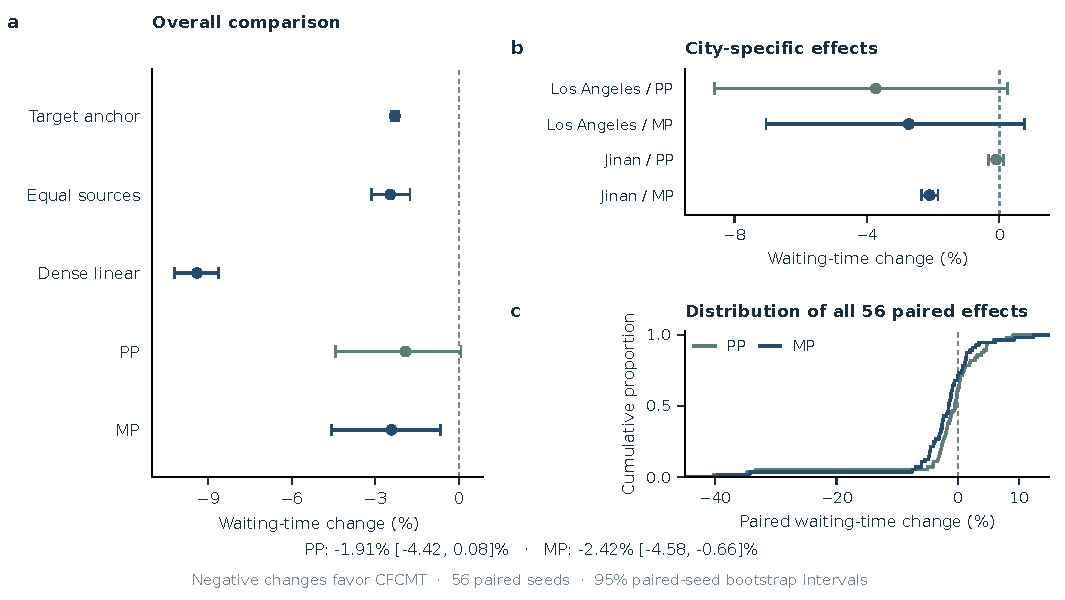
\includegraphics[width=\textwidth]{source_selector_with_mp.pdf}
\caption{Frozen source selection on 56 paired simulation replicates. (a) Mean city-wise relative waiting changes and 95\% paired bootstrap intervals against all five comparators. (b) City-specific mean changes and intervals against PhasePressure (PP) and MaxPressure (MP). (c) Empirical cumulative distributions of all 56 equal-city paired changes against the two pressure rules. At zero, each curve gives the fraction of nonpositive relative changes. Negative values favor \method.}
\label{fig:comparisons}
\end{figure*}

Against PhasePressure, the registered mean change is $-1.91\%$, with interval $[-4.42,0.08]\%$ and 34 favorable seed means. The city-specific changes are $-3.73\%$ for Los Angeles and $-0.10\%$ for Jinan. Its equal-city interval crosses zero. Figure~\ref{fig:comparisons} shows the comparator intervals, city-specific effects, and the full distributions of paired changes against both pressure rules.

\subsection{Source selection and learned comparators}
Against the target anchor, equal source weights, and the frozen dense linear baseline, the corresponding relative changes are $-2.30\%$, $-2.46\%$, and $-9.40\%$, respectively; all three paired intervals exclude zero. The selected controller exactly matches the target anchor in Los Angeles and improves on it by 4.60\% in Jinan, with all 56 Jinan seed means favorable. The raw equal-city waiting means in Table~\ref{tab:source-selector} and the registered mean relative changes summarize the same complete runs with different weighting: taking a ratio after pooling the waiting values gives greater weight to large Los Angeles values.


\section{Discussion}
\subsection{What the results establish}
The frozen source selector improves the paired-seed waiting outcome over MaxPressure in the two-network comparison. Its Jinan improvement over the target anchor and exact fallback to that anchor in Los Angeles support the tested source-selection procedure. The favorable PhasePressure point estimate gives a less conclusive comparison because its interval crosses zero.

The main comparison supports the tested predictor configuration over the dense linear residual baseline. It does not show that every component is necessary. In particular, the gain may reflect the nonlinear regressor, action normalization, feature restrictions, pairwise learning, weighting, or their interaction. A capacity-matched nonlinear baseline and controlled component ablations are needed before attributing the effect to a specific architectural choice.

\subsection{Training and deployment}
There are two changes between the supervised task and deployment. First, the labels measure one focal phase choice followed by PhasePressure, with other intersections also using PhasePressure. The deployed controller repeatedly chooses learned phases at multiple intersections. It can therefore visit states and joint action combinations that differ from those under the label continuation. Second, the training target is a 60-s vehicle-load measure, whereas evaluation measures waiting and completion over an hour. An action can improve the former without improving the latter. These differences can limit how offline regret predicts closed-loop waiting, but the present experiments do not identify their individual causal contributions.

\subsection{Scope of the evidence}
Controller selection uses eight target closed-loop development seeds, and the evaluation tests the complete fitting and execution procedure. The anchor and source component also differ in model capacity. It therefore measures the complete selection procedure, rather than an isolated benefit of source data or any single component. The city-specific MaxPressure interval still crosses zero for Los Angeles; the confirmed aggregate effect is not a separate confirmation in every city.

The external study contains two geometries. Three demand files for Jinan and additional random seeds increase coverage within those geometries; they do not increase the number of independent cities. Target-network diagnostics were used during development, although the reported final seeds were withheld. The simulator is not calibrated to field trajectories, and both adaptation and evaluation use the same physics engine. We therefore cannot infer physical deployment performance, robustness to a different simulator, or effectiveness under detector failure and unobserved demand regimes.

The word ``causal'' in the method's name refers to controlled simulator interventions and predefined input restrictions. It does not claim observational causal discovery or invariance in the physical network. Similarly, heuristic error scores do not certify safety.

Finally, same-protocol comparisons with transfer methods such as CrossLight, X-Light, GESA, and MetaLight remain missing. An informative next evaluation would match model capacity and target information, use the same signal executor, and include additional networks withheld from method development. It should test target-only and source-aware training with identical architectures and measure both short-horizon action quality and sustained closed-loop behavior. That design would distinguish a useful representation from a demonstrable benefit of transferred data.

\section{Conclusion}
We presented a supervised method for adapting signal control across road networks by learning differences between feasible phase choices. A restricted reference predictor and an antisymmetric pairwise predictor are combined using target simulation data, then deployed without online refitting. The final controller selects source components or a target anchor using eight target development seeds before freezing its predictors and execution guard. On 56 paired seeds across two target networks, it reduces mean city-wise relative waiting by 2.42\% against MaxPressure, with a 95\% reduction interval of 0.66--4.58\% and 40 favorable seed means. It also lowers waiting relative to the tested target anchor and dense linear residual baseline. The PhasePressure point estimate is favorable, but its interval crosses zero. The evidence supports the complete source-selection procedure on these fixed networks and motivates capacity-matched tests of the source data's contribution on additional independent networks.

\section*{Data and Code Availability}
\begingroup\raggedright
The source-component fitting and deployment code are available in the CFCMT repository at commit \texttt{61e8a81}.\footnote{\url{https://github.com/erzhu419/CFCMT}, commit \texttt{61e8a81}.}
The accompanying source-data files contain all 1,344 runs of the six-controller comparison and their paired summaries. The fixed-baseline MaxPressure execution and analysis scripts are in \path{experiments/tsc_v93_max_pressure_20261030}.
The exports support the numerical summaries reported here. Full simulation logs, trained models, and some aggregated evaluation records remain in the execution archive and are not all included in this repository snapshot. The release therefore does not yet provide an end-to-end reproduction package. The benchmark inputs retain their upstream licences.
\par\endgroup
\section*{Acknowledgment}
OpenAI ChatGPT assisted with the organization and English drafting of the abstract and Sections I--VIII, and with preparation of the figures and tables. Codex assisted with the supplemental evaluation and analysis scripts. Simulation outcomes were produced by SUMO using the frozen controllers.
\appendices
\section{Source-Component Details and Score Properties}
\label{app:score-proofs}


\emph{Los Angeles source-component configuration.}
The source candidates and equal-source comparator in Los Angeles use the
following fixed blend rule. Let $a_A$ and $a_P$ minimize $A_g$ and $P_g$,
respectively. The operator $\range$ denotes the maximum minus the minimum of a score over feasible actions. Then
\begin{align}
 h_g&=\max\{\range(A_g),\median_a u_{A,g}(a),10^{-6}\},\nonumber\\
 D_g&=\range(P_g-A_g)/h_g,\nonumber\\
 M_g&=\max\{P_g(a_A)-P_g(a_P),0\}/h_g,\nonumber\\
 U_g&=\{u_{P,g}(a_A)+u_{P,g}(a_P)\}/h_g,\nonumber\\
 \alpha_g&=\min\{1,1/\max(D_g,10^{-12})\}\nonumber\\
 &\quad{}\times\ind\{M_g+10^{-12}\geq0.25U_g\}.
 \label{eq:la-component-blend}
\end{align}
Here $h_g$ is the reference-score scale, $D_g$ is normalized model
disagreement, $M_g$ is the pairwise margin, and $U_g$ is the combined error
score. The operator $\median$ takes the median over feasible actions, and
$\ind$ is one when its condition holds and zero otherwise. The final Los
Angeles controller selects the target anchor rather than these source
components.

\emph{Common-offset cancellation.}
Subtracting $Y_g(r_g)$ from $Y_g(a)$ cancels $b_g$ and gives
\eqref{eq:cancellation}. Adding a common constant leaves every contrast and
the group range unchanged. Multiplying all outcomes by a positive constant
multiplies both by that constant, so normalized labels are unchanged when
the numerical floor is inactive. Action ordering is preserved in either case.

\emph{Pairwise ranking recovery.}
Swapping $i$ and $j$ in \eqref{eq:antisym} negates the prediction. For exact
pair predictions,
\begin{equation*}
 \sum_{j\ne i}\{z_g(a_i)-z_g(a_j)\}
 =K_gz_g(a_i)-\sum_{j=1}^{K_g}z_g(a_j).
\end{equation*}
Dividing by $K_g-1$ and subtracting the reference score gives
\eqref{eq:recovery}. The common subtraction and positive factor preserve
the minimizers, and $P_g(r_g)=0$.

\emph{Ranking error.}
For the ranking bound, let $a_g^\star$ minimize $z_g$. By the definition of
$\widehat a_g$ in \eqref{eq:blend},
\begin{align*}
 z_g(\widehat a_g)-z_g(a_g^\star)
 &=z_g(\widehat a_g)-S_g(\widehat a_g)\\
 &\quad+S_g(\widehat a_g)-S_g(a_g^\star)\\
 &\quad+S_g(a_g^\star)-z_g(a_g^\star)\\
 &\leq2\|S_g-z_g\|_\infty.
\end{align*}
Here $\|S_g-z_g\|_\infty$ is the largest absolute score error over the feasible
actions. This is an algebraic bound; it assumes no error guarantee for an
unseen network.

\bibliographystyle{IEEEtran}
\bibliography{references}
\end{document}
